% \section*{Appendix A: Proof of Kepler's Laws}
% \addcontentsline{toc}{section}{Appendix A: Proof of Kepler's Laws}
% As a reminder, here is a restatement of Kepler's Laws:\\
% 1. All planets orbit around a sun in elliptical orbits with the sun at one focus of the ellipse.\\
% 2. Planets sweep out equal-sized areas in equal time intervals. \\
% 3. The square of the period of a planet's orbit around a mass $M$ is proportional to the cube of the semi-major axis of the planet's orbit: more specifically, 
% \[
% 	T^2 = \frac{4\pi^2}{GM} a^3
% \]
The first and third statements follow from Newton's Law of Universal Gravitation, but the second is essentially a disguised conservation of angular momentum (see the problems from Rotation!). We're going to prove these two using Newton's Law of Universal Gravitation and Newton's Second Law of Motion. \\
\begin{center}
	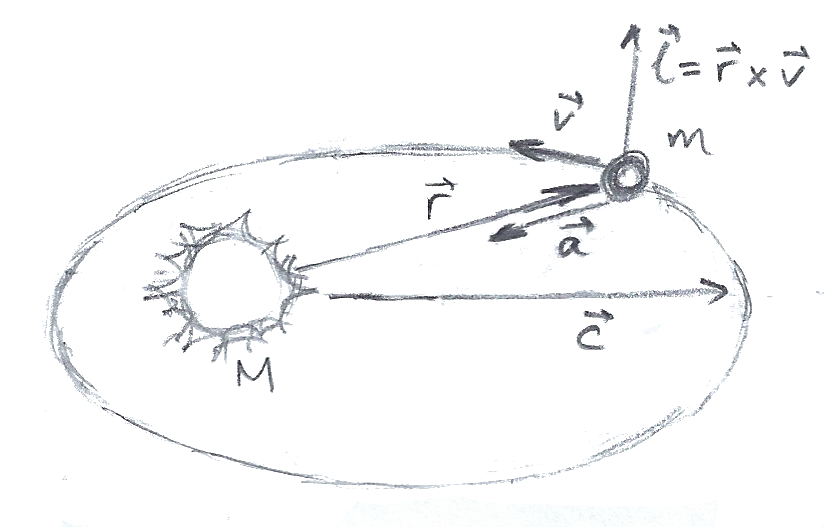
\includegraphics[width=0.5\textwidth]{images/mechintro/kepler-1.png}\\
\end{center}
If a satellite of mass $m$ is orbiting around a mass $M$, the force $\vec F = - \frac{GmM}{r^2} \hat r$ where $\hat r$ and $r$ are varying with time. Because of this, notice that $\vec a =  - \frac{GM}{r^2} \hat r$ from Newton's Second Law. The position $\vec r$ and $\vec a$ are then always in the same direction. \\
Assuming no other forces act on the system, the orbital angular momentum $\vec L = \vec r \times m \vec v$ is constant. We're more interested in the fact that the cross product $\vec r \times \vec v$ is also a constant, so we're going to denote this by $\vec l$. But what exactly is $\vec l$? We can do this explicitly:
\begin{align*}
	\vec l &= \vec r \times \vec v \\
	&= \vec r \times \dv{\vec r}{t}\\
	&= r \hat r \times \dv{}{t}(r \hat r)\\
	&= r \hat r \times (r' \hat r + r \hat r')\\
	&= r^2(\hat r \times \hat r')\\
\end{align*}
We're going to do something a little contrived: what happens when we take $\vec a \times \vec l$? We can use the triple vector product identity to help us out, and the fact that we've decomposed everything into unit vectors with magnitude 1:
\begin{align*}
	\vec a \times \vec l &=  - \frac{GM}{r^2} \hat r \times r^2 (\hat r \times \hat r')\\
	&= -GM [ \hat r (\hat r \cdot \hat r') - \hat r' (\hat r \cdot \hat r) ]\\
	&= GM \hat r'
\end{align*}
The first dot product in parentheses is zero - the derivative of a unit vector is always perpendicular to the original. If you're not convinced, look at $\hat r$ and $\hat \theta$ when we derived circular motion - $\hat \theta$ is proportional to the derivative of $\hat r$, and $\hat \theta \cdot \hat r = 0$. \\
Since we know how $\vec a \times \vec l$, we can find $\vec v \times \vec l$. Considering that 
\[
	\dv{}{t} (\vec v \times \vec l) = \dv {\vec v}{t} \times l + \vec v \times \dv{\vec l}{t} = \vec a \times \vec l + \vec v \times \vec 0 = \vec a \times \vec l
\]
we can integrate to find $\vec v \times \vec l = GM \hat r + \vec c$ for some constant vector $\vec c$. \\
We have one more contrived step to take: consider $\vec r \cdot (\vec v \times \vec l)$. We can expand it as follows:
\begin{align*}
	\vec r \cdot (\vec v \times \vec l) &= \vec r \cdot (GM \hat r + \vec c) \\
	&= GM (\vec r \cdot \hat r) + \vec r \cdot \hat c\\
	&= GMr + rc \cos \theta
\end{align*}
where $\theta$ is the angle between $\vec r$ and $\vec c$. On the other hand, since this is a scalar triple product, $\vec r \cdot (\vec v \times \vec l) = \vec l \cdot (\vec r \times \vec v) = \vec l \cdot \vec l = l^2$. Therefore, 
\[
	l^2 = GMr + rc \cos \theta
\]
\[
	r = \frac{l^2}{GM + c \cos \theta} = \frac{\frac{l^2}{GM}}{1 + \frac{c}{GM} \cos \theta}
\]
That is the polar equation for an ellipse, centered at one of its foci (if you might recall from the conics unit), and this gives Kepler's First Law.\\
\begin{center}
	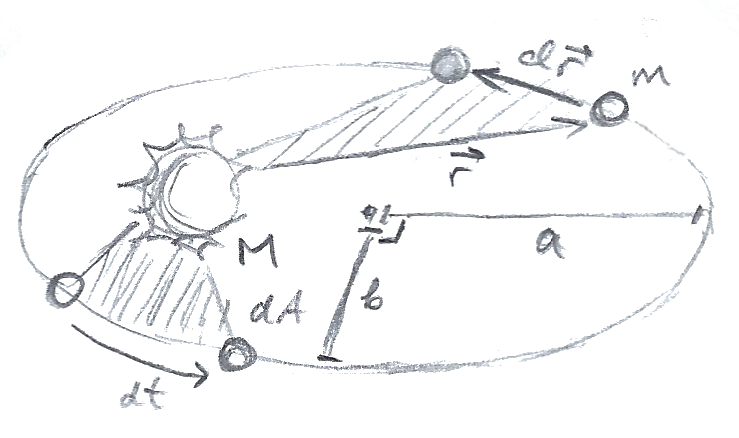
\includegraphics[width=0.5\textwidth]{images/mechintro/kepler-2.png}\\
\end{center}
For Kepler's Second Law, we reuse the fact that $\vec l = \vec r \times \vec v$ is a constant. Consider a small triangular area $dA$ swept out in a time $dt$ by a satellite. This area $dA = \frac{1}{2}| \vec r \times d\vec r |$, where $d\vec r$ is the displacement of the satellite. Dividing by $dt$ gives $\dv{A}{t} = \frac{1}{2} \left| \vec r \times \dv{\vec r}{t} \right| = \frac{1}{2} \left| \vec r \times \vec v \right| = \frac{1}{2} l$. Since $\vec l$ is constant, we have that the area swept out per unit time is constant, so the area swept out by a satellite in a given time interval is also a constant. \\
Using this, we can prove Kepler's Third Law. The rate at which area is swept out is $\dv{A}{t} = \frac{1}{2} l$ by Kepler's Second Law, but since this is constant it's also equal to the total area of the elliptical orbit over the period of the motion. Letting $a$ and $b$ be the lengths of the semi-major and semi-minor axes, we have 
\[
	\dv{A}{t} = \frac{\pi a b}{T} = \frac{1}{2}l
\]
From this, we see that 
\[
	T = \frac{2\pi a b}{l} \rightarrow T^2 = \frac{4\pi^2 a^2 b^2}{l^2}
\]
I'm going to gloss over this part a little bit - but recall that an ellipse in polar coordinates is defined by its eccentricity $e$ and the distance from the focus to the directrix $d$. The computation is extremely messy, but it can be shown (with great effort) that the numerator of the polar equation $ed = \frac{b^2}{a}$. In this case, then, $\frac{l^2}{GM} = \frac{b^2}{a}$, which is equivalent to $\frac{b^2}{l^2} = \frac{a}{GM}$. We can plug this back in to get
\[
	T^2 = \frac{4\pi^2}{GM}a^3
\]
This shows Kepler's Third Law. Usually, however, we won't work with actual elliptical orbits - most of the time we will just deal with simplified circular orbits, where the semi-major axis is just the radius of the circle. 